\documentclass[letterpaper, 12pt, conference]{ieeeconf}
% piazza says 12pt

\usepackage[utf8]{inputenc} % allow utf-8 input
\usepackage[T1]{fontenc}    % use 8-bit T1 fonts
\usepackage{hyperref}       % hyperlinks
\usepackage{url}            % simple URL typesetting
\usepackage{booktabs}       % professional-quality tables
\usepackage{amsfonts}       % blackboard math symbols
\usepackage{nicefrac}       % compact symbols for 1/2, etc.
\usepackage{microtype}      % microtypography
\usepackage{graphicx}
\usepackage{verbatim} % comments
\usepackage[ruled]{algorithm2e} % alg wrapper
\usepackage{amsmath}


\usepackage[
    backend=biber,
    style=alphabetic,
    sorting=ynt,
    style=ieee
]{biblatex}
\addbibresource{references.bib}

\title{Improving New Editor Retention on Wikipedia}
\author{Jonathan Hollenbeck \\ 
    \href{jonoh@stanford.edu}{jonoh@stanford.edu} 
\and Anthony Miyaguchi \\
    \href{acmiyaguchi@stanford.edu}{acmiyaguchi@stanford.edu}}
  
\begin{document}
\maketitle

\begin{abstract}
We consider impacts to continued participation by new Wikipedia editors. We frame this as a prediction problem, where we model whether a new user will become an established member of the community based on their initial activity. This is a proxy; we are primarily interested in determining positive and negative impacts to new user retention. To derive a base model, we draw inspiration from previous work, especially analysis\cite{burke2008mopping}\cite{leskovec2010governance} of the site's administrative promotion process, to build features from each user's first quarter of activity. We compute target values based on contribution level in their second quarter, then regress to evaluate a baseline model. We then compare the base model against an extended feature set with role and community attributes. Finally, we draw conclusions about the importance of network features by comparing the extended and base models, and observe which individual metrics matter most.

\end{abstract}

\section{Introduction}
Large open source projects need to recruit new volunteers to sustain and grow. However, user retention often clashes with established cultures and the maintenance of community norms. As an example of this, Wikipedia meta-lore\cite{wiki:deletionism} describes scenarios where prospective editors struggle to understand standards and clash with diligent maintainers, eventually leaving the project after a series of negative experiences. Nobody enjoys seeing their good-faith contribution reverted, even when justified by community guidelines. In this project, we explore the interactions experienced by new Wikipedia editors in terms of graph properties, and evaluate them by regressing against a retention metric. We hoped to suggest concrete guidelines and actionable tools for the site to improve recruitment of new prospective editors, but in general did not discover significant novel observations.

\section{Related Work}
Wikipedia promotes established, self-nominated editors to administrators through a Request for Adminship (RfA), an open community voting process concluded by an arbiter. Drawing on community guidelines for prospective admins\cite{wiki:rfa}, Burke\cite{burke2008mopping} builds diverse feature sets to represent specific criterion from the guidelines, then regresses against a probit model to predict the outcomes of historical promotion processes. The paper focuses on utilizing this as a tool for editors to gauge readiness, and for the community to automatically discover candidates, but also notes feature significance. Leskovec\cite{leskovec2010governance} models the same problem, but focuses on candidate-voter similarity and notes a strong correlation between high similarity and 'yes' votes.

Observing the Q\&A site StackOverflow, Anderson\cite{anderson2012discovering} tackles two separate problems: predicting whether a question has been sufficiently answered, and whether it has long-term value. Suggesting a change of mindset, they focus on the significant features instead of model performance, emphasizing a motivation to improve the general design of Q\&A sites. We find this approach compelling, since we are primarily interested in making recommendations based on significant features. Furthermore, generating features from network analysis of the Q\&A process proved fruitful, suggesting that considering interactions can be critical to understanding community behavior.

Structural signatures and behavior have been used to analyze social roles\cite{welser2011finding} within the Wikipedia ecosystem. The interactions between roles and the composition of communities may provide context around user retention. RolX\cite{henderson2012rolx} achieves role assignments that can improve classification accuracy on various tasks by recursively aggregating features of the local network and clustering through non-negative matrix factorization.

Community detection may also play a role in predicting new user outcomes, particularly as a normalizing factor. AGMfit\cite{leskovec2016snap} seems promising for this task, since it generates probabilistic community memberships. We also utilize various binary classification algorithms, especially Spectral Clustering and Louvain\cite{louvain2008}.

\section{Data}

We utilize the parsed Wikipedia edit history data available in the SNAP repository. The compressed metadata is 8GB with 116M edits over 7 years and includes 11M users and 2.9M articles. Each edits maps to a row with the following columns:

\begin{table}[ht]
    \caption{Edit Data Examples}
    \label{tab:edit_data}
    \centering
    \begin{tabular}{c|c|c|c|c|c}
        \toprule
    Article & User & Words & Minor & Timestamp \\
        \midrule
        10 & 99 & 8 & false & 2001-01-20 18:12:21 \\
        454 & 600 & 663 & false & 2001-01-22 05:09:05 \\
        \bottomrule
    \end{tabular}
\end{table}

We represent the contribution network as a series of time-delimited snapshots. Each snapshot is a bipartite user-article graph built up from all included edits, where an edit creates an edge between the user and article. A given snapshot $p \in P$ includes all data with timestamp t such that $t_p \leq t < t_p + T $. We choose a period of a quarter (or three calendar months) since it provides a balance between the length of the entire data-set and the number of events that occur within the snapshot. 

To clean the set of users we make predictions on, we removed all users with 'ip:' in the User ID, since these denote unregistered users whom we cannot reliably identify over time. We also remove all users with case-insensitive 'Bot' in their username, since this marks automated accounts by convention. This second condition is not a comprehensive filter, since bots can register under any name, operate anonymously, or run within an established user account. This exclusion was only done for the prediction task: we did not exclude any data from the bipartite graph or its projections, since interactions with anonymous users and robots may impact the new user experience.

This representation has two major flaws. The first is the inability to distinguish specific behaviors from an unsigned word count of additions and deletions. Second, the snapshot approach is an approximation of a better temporal graph representation. We would prefer to observe a new user through an aligned snapshot from $t_0$ to $t_0+T$, where $t_0$ is their registration date.

Most Wikipedia distributions (Figure~\ref{fig:distributions}) follow an approximate power-law distribution. Edit sizes are one important exception that tend to peak around 200-300 words, since common forms of contributions add blocks of content or new articles. This also causes the peak in total user words that is not observed in the user edit counts. We suspect that the registration process also impacts the total word count -- users may be more likely to register when they want to get credit for new work.

\begin{figure}[ht]
    \centering
    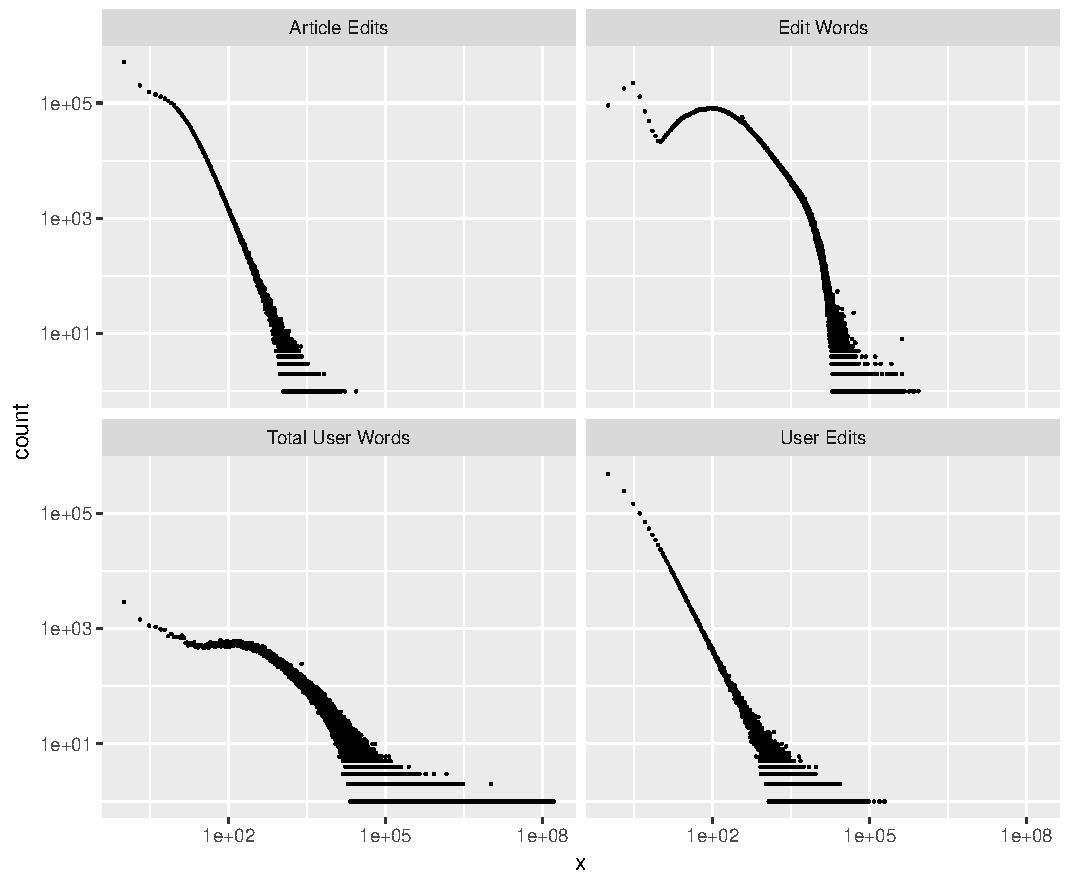
\includegraphics[width=1\linewidth]{dist_segment.pdf}
    \caption{Edit Data Distributions}
    \label{fig:distributions}
\end{figure}

We use uni-modal projections of network snapshots to build features. The user-user network is constructed by adding edges between users if they both contribute to the same article. Likewise, edges in the article-article network represent shared contributors. A projection captures indirect interactions between entities by proximity, compensating for the lack of direct relationships between nodes of one type. Formally, given an $n \times m$ adjacency matrix A of n users and m articles, the user projection is $AA^T$ and the article projection is $A^TA$. The entry $U_{ij}$ of the user network is an edge between user $i$ and user $j$. The baseline projection (Table II) is a densely connected graph.

\begin{table}[ht]
    \centering
    \label{tab:uu_proj_stats}
    \caption{User Projection Graph (2007-Q1)}
    \begin{tabular}{c|c|c|c|c}
        \toprule
        Graph & Nodes & Edges & Density & C \\
         \midrule
        Bipartite & 1.35m U, 1.8m A & 7.53m & 2.39 & 0 \\
        User-User & 116k U & 7.56m & 65.33 & 0.67 \\
         \bottomrule
    \end{tabular}
\end{table}

The base projections generate a large number of edges, causing high clustering among active users. In the article-article case, this generates an intractable number of edges (over 1 trillion by weight). Cliques are the root cause of this issue -- if 1000 users edit the same article, we will form a 1000-clique with almost half a million edges. However, even minimal thresholding techniques (see section on Null Results) disconnect most of the new contributors with low levels of participation, and simultaneously create very dense cliques between active editors. Other standard thresholds, such as Jaccard similarity, faced similar issues.

To resolve this tradeoff, we propose two sampling techniques, which operate directly on cliques. Given some probability p, the chance of any user in a clique of size k staying connected (retaining at least one edge) is:
\begin{equation}
    P(X_{any} \geq 0) 
    = 1 - (1-p)^{(k-1)} 
    \geq 1 - \epsilon
\end{equation}
Similarly, the chance that all users in a clique of size k will retain at least one edge is:
\begin{equation}
    P(X_{all} \geq 0)
    = (1-(1-p)^{(k-1)})^{(k)}
    \geq 1 - \epsilon
\end{equation}

The first bound tends to generate edges roughly proportional to the number of edges in the original projection, and the latter places greater weight on larger cliques (see Table \ref{tab:proj_sampling}). Also note the logical similarity to S-curves from LSH-clustering.\cite{leskovec2014mining}

\begin{table}[ht]
    \centering
    \begin{tabular}{c|c|c|c|c}
        \toprule
        k & $p_{any}^*$ & $p_{all}^* $ & Edges/User (any) & Edges/User (all) \\
        \midrule
        2 & .99 & .995 & .99 & .995 \\
        5 & .602 & .722 & 3.01 & 3.61 \\
        10 & .369 & .505 & 3.69 & 5.05 \\
        100 & .045 & .088 & 4.5 & 8.8 \\
        1000 & .0046 & .0155 & 4.6 & 15.5 \\
        \bottomrule
    \end{tabular}
    \caption{Bounded Clique Sampling for $\epsilon=0.01$}
    \label{tab:proj_sampling}
\end{table}

To run projection sampling, we first group edits into sets of users who contributed to a common article during a snapshot (for articles, we group edits within a snapshot by articles with common users). These form cliques in the user-user projection. This results in a strictly smaller list, since any one contribution can only appear in one set. Then, we generate a portion of the edges in the clique, based on its size (see \ref{tab:proj_sampling}). Implementing this is straightforward in SQL, Spark, or any MapReduce framework. 

\begin{table}[ht]
    \centering
    \begin{tabular}{c|c|c|c}
        \toprule
        Graph & Nodes & Edges & CC \\
        \midrule
        Bipartite & 53.6m & 1.52m U, 2.92m A & 0 \\
        User & 1.52m & 282m & - \\
        User (Sampling) & 1.52m & 34.8m & 0.40 \\ 
        Article & 2.92m & 47.0b & - \\
        Article (Sampling) & 2.92m & 89.7m & 0.028 \\
        \bottomrule
    \end{tabular}
    \caption{Unimodal Graph Projections}
    \label{tab:graph_projections}
\end{table}

The unimodal projections roughly follow the degree distribution of the original projections (see Figure~\ref{fig:proj_vs_bipartite}). This is expected, but definitely not guaranteed for the general case. For both projections, we note a curvature near the top of the graph. This happens because we generate 3-4 edges per user or article for most cliques (see Table~\ref{tab:proj_sampling}), so even if a node only has one edge in the bipartite graph, they tend to have a few edges in the projections.

% need to cleanup
\begin{figure}[ht]
    \centering
    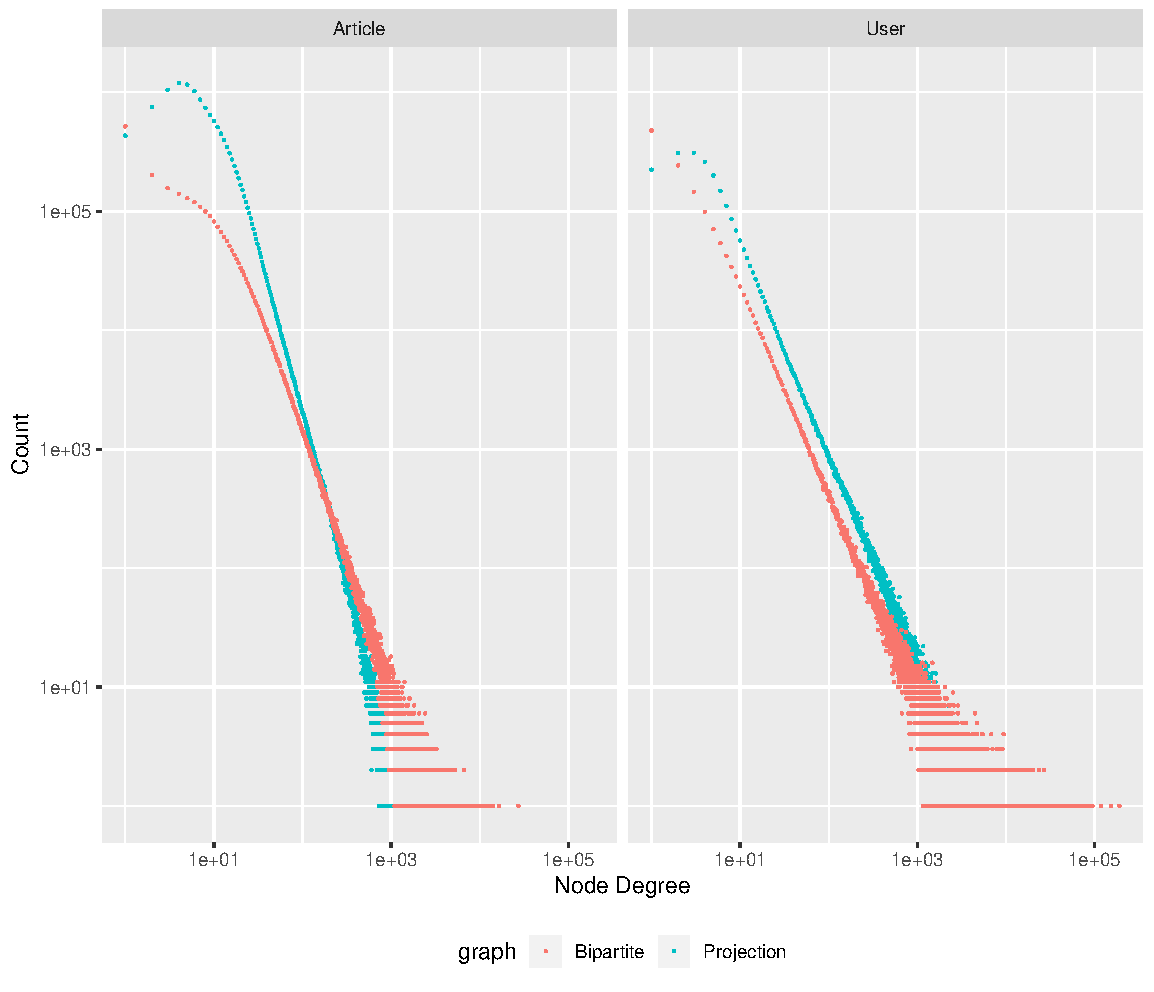
\includegraphics[width=1\linewidth]{proj_vs_bipartite.pdf}
    \caption{Degree Distributions: Bipartite vs. Projection}
    \label{fig:proj_vs_bipartite}
\end{figure}

\section{Model}

We define the prediction problem as follows: given information about a new user i in snapshot p, predict their contribution level $y_i^{(p)}$ in snapshot p+1. We justify this by observing patterns in the lifespan of an account: while large proportion of users drop out quickly, retention is quite high for users who stick around past 100 days (Figure~\ref{fig:account_duration}). Note that account lifespans are left-skewed because users may continue to participate in the future.

\begin{figure}[ht]
    \centering
    \includegraphics[width=1\linewidth]{account_duration.pdf}
    \caption{Account Lifespan}
    \label{fig:account_duration}
\end{figure}

Based on the empirical distribution, we define contribution for a user as follows:
\begin{equation}
    y_u = \sum_{e \in E(u)} log(1+e_{words})
\end{equation}
This is intended to smooth out contribution weighting, while still somewhat favoring larger contributions. Without taking $log(x)$, we found that single large contributions were overemphasized, since a 1000 word article would equal 50 small 20 word edits. We also regress and evaluate the model against $log(y)$, since this definition of contribution follows a power law.

We then generate three blocks of data: baseline, role, and community features (B + R + C). The baseline features are built with SQL, drawing inspiration from previous work\cite{burke2008mopping}\cite{leskovec2010governance}\cite{anderson2012discovering}. We use a variety of indicators for this, but specifically do not consider graph interactions beyond the egonet. Based on the user network, we compute roles in each snapshot and average role interactions for each new user. Finally, we compute a set of community memberships from the article network, statistics about each community, and build up in and out-community interaction features for each user. We regress each element of the power set of baseline, role, and community features against the labels, using gridsearch on an l2-regularized neural net in scikit-learn. For a more formal description, see Alg~\ref{alg:ml}.

The results in all cases tend to follow a hedging paradigm (Figure \ref{fig:hedging}), where we consistently under-predict user contribution, since there is a large chance that users will not return, regardless of their contribution level. This is analogous to predicting house prices when the house may disappear at random. Current ML models are perfectly capable of calibrating to this problem, but we found it extremely difficult to interpret. 

For this reason, we broke the problem into two parts: classification (will the user contribute anything?) followed by regression (given that the user contributed something, how much did they contribute?). We can then multiply these together to approximate the full model. Specifically:

\begin{equation*}
     \hat{y} = E[y] 
    = E[y|\theta]P(\theta) + E[y|\bar{\theta}](P(\bar{\theta})) 
\end{equation*}
\begin{equation}
    = E[y|\theta]P(\theta)
\end{equation}

The last step follows because $E[y|\bar{\theta}] = 0$. We can now iterate on classification ($P(\theta)$) and regression ($E[y|\theta]$) separately, then use the results to improve the original model. This is not guaranteed to find the optimal solution, but in practice, this combined model was extremely close in performance to the independently built full model. 
% As an aside, this also helped us catch data leakage errors, since combined model performance on $\theta=0$ samples was extremely poor if we memorize while building the regression model.

% might want to mention not rebalancing for classification, since that's a bit non-standard. or, figure out how to rebalance.
We evaluate with standard techniques: log-loss for classification, and $R^2$ score for regression.

\section{General Approach}

We followed a general procedure (Alg~\ref{alg:ml}) to generate sets of Baseline, Role, and Community features X, and compare their efficacy in predicting a target variable y. 
We especially compare performance with $B$ to $X$ (B + R + C) to evaluate the added information from the graph-based approach.

\begin{algorithm}[ht]
    \label{alg:ml}
    \caption{A generic feature mining procedure}
    \SetAlgoLined\SetArgSty{}
    \SetKwInOut{Input}{input}
    \Input{ K-partite Graph $G \in \mathcal{R}^{n \times m}$ }
    \ForEach{Period $p \in P(G)$}{
        compute snapshot $G^{(p})$ from G \\
        compute baseline features $B^{(p)} \in \mathcal{R}^{n \times b}$ \\
        \ForEach{Node type $k \in G$}{
            compute unimodal projection $G_k^{(p)}$ \\
            reduce $G_k^{(p)}$ density with bounds \\
            %run RolX on $G_k^{(p)}$, get features $R_k^{(p)}$ \\
            $R_k^{(p)} := \text{RolX}(G_k^{(p)}) \in \mathcal{R}^{n 
            \times r}$ \\
            %run Louvain on $G_k^{(p)}$, get features $C_k^{(p)}$ \\
             $C_k^{(p)} := f( \text{Louvain}(G_k^{(p)})) \in \mathcal{R}^{n \times  c}$
             % aggregated features
        }
        % column stack R,C (add nesting?)
       $R^{(p)} :=
           \begin{bmatrix}
           R^{(p)}_1 & R^{(p)}_2 & \hdots & R^{(p)}_k
           \end{bmatrix}$ \\
       $C^{(p)} := 
           \begin{bmatrix}
           C^{(p)}_1 & C^{(p)}_2 & \hdots & C^{(p)}_k
           \end{bmatrix}$ \\
       $X^{(p)} := 
            \begin{bmatrix}
            B^{(p)} & R^{(p)} & \hdots & C^{(p)}
            \end{bmatrix}$ \\
   }
    % row stack features (why error?)  
    $X := \begin{bmatrix}
    X^{(1)T} & X^{(2)T} & \hdots & X^{(P)T} 
    \end{bmatrix}^T$ \\
    $= \begin{bmatrix}
        B & R & C
    \end{bmatrix}$ \\ 
    compute $y$, where $y^{(p)}$ in $B^{(p+1)}$ \\
    \SetKwInOut{Output}{output}
    \Output{features X, target y}
\end{algorithm}


\section{Baseline Features}

First, we collected simple features to describe individual users, roughly grouped into categories (Table~\ref{tab:user_features}).

\begin{table}[ht]
    \centering
    \caption{Baseline User Features}
    \begin{tabular}{c|c|c}
        \toprule
        Category & Features & Example \\
        \midrule
        Magnitude & 6 & Log of Total Word Count \\
        Timing & 4 & Time since Last Active \\
        Ratios & 4 & \% Minor Revision \\
        Type Counts & 4 & Distinct Articles \\
        Total & 18 \\
        \bottomrule
    \end{tabular}
    \label{tab:user_features}
\end{table}

We also build a set of features, $A$, defined for each article over a quarter. For each user i and article feature j, we average the feature over edits e in the user's edit set $E^{(i)}$:
\begin{equation}
    x^{(i)}_j = \frac{1}{|E^{(i)}|} \sum_{e \in E^{(i)}} A^{(e_{article})}_j
\end{equation}
These are also grouped into categories (Table~\ref{tab:article_features}).

\begin{table}[ht]
    \centering
    \caption{Baseline Article Features}
    \begin{tabular}{c|c|c}
        \toprule
        Category & Features & Example \\
        \midrule
        Magnitude & 4 & Total Edit Count \\
        Average & 4 & Edits per Unique User \\
        Ratio & 5 & \% Edits from IP User \\
        Type Count & 5 & Total Bot Edits \\
        Total & 18 \\
        \bottomrule
    \end{tabular}
    \label{tab:article_features}
\end{table}


\section{Role Features}

We use graph role mining to generate mapping of nodes to roles defined by local structural properties of the network. Mining on the original contribution network would require modifications to account for the bipartite structure, so we instead work with the user projection. Recursive feature extraction on this captures each user's relationship to others in terms of local structure. Using Snap\cite{leskovec2016snap}, we collect a recursive feature-set $V \in \mathcal{R}^{n \times f}$, where $n = \text{number of users}$ and $f = \text{number of features}$. This ReFex feature vector \cite{henderson2011s} is then used within our model after running a truncated SVD. We then analyze the distribution of roles across users, neighborhoods, and communities through RolX sensing techniques.

We observe the properties of $V$ on the user network for the first quarter of 2007 with 342k users associated with a 44-dimensional ReFex vector. Roles are found by finding a low-dimension space such that $G \cdot F \approx V$, where $G$ is a mapping of user to roles and $F$ is a mapping of roles to features. A singular value decomposition (SVD) finds a single dimension that captures $99.4\%$ of variance, which means that roles are primarily encoding magnitude of contribution. We also run a soft-clustering procedure through non-negative matrix factorization (NMF) to interpret the vectors separately from the model.

The number of roles in RolX is found by balancing the number of roles against improvement in a cost function. A grid-search tends to select many roles, despite limited utility, so we fix the number of roles at 8. 
We then assign users a discrete role by magnitude and generate aggregate statistics for each role. Most users are contained in roles 0-2 (Figure~\ref{fig:uu_proj_roles}). We run RoleSense to determine the correlation between each role and our contribution regression target in Figure~\ref{fig:nodesense}; roles 3 and 6 exhibit a higher contribution by orders of magnitude. We found that these two roles contain more administrators per capita at $9.6\%$ and $5.2\%$ respectively, compared to the next highest role, 1, at $0.14\%$. This result aligns with the significantly higher than average contribution level of administrators in the network, and also demonstrates a high level of indirect interactions between admins.

\begin{figure}
    \centering
    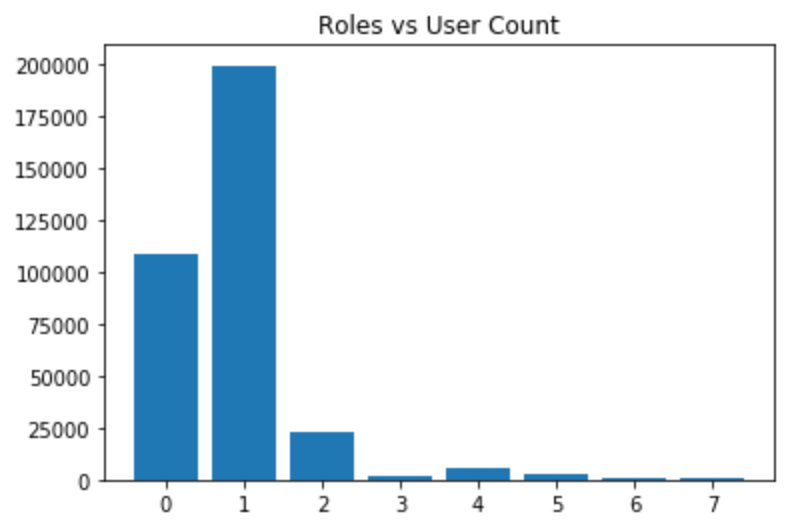
\includegraphics[width=1\linewidth]{role_counts.png}
    \caption{User Network Roles (2007-Q1)}
    \label{fig:uu_proj_roles}
\end{figure}

\begin{figure}
    \centering
    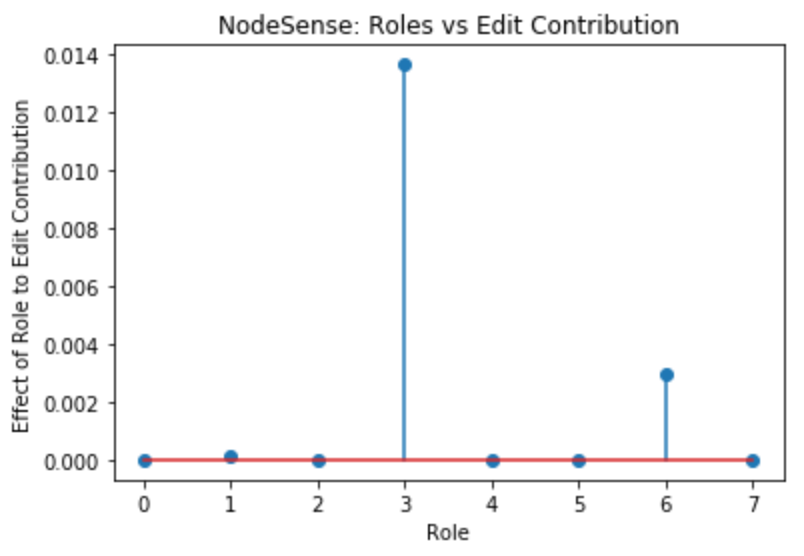
\includegraphics[width=1\linewidth]{nodesense.png}
    \caption{A plot of role-significance to edit contribution normalized by contribution assuming a single role.}
    \label{fig:nodesense}
\end{figure}

We also analyze the distribution of roles across neighborhoods by computing role interactions between neighbors. Specifically, given a role vector $r_i$ for each user i, where $1^T r_i = 1$, we calculate the role interaction vector $x_i$ as follows:

\begin{equation}
    x_i = \frac{1}{|N(i)|} \sum_{k \in N(i)} r_k
\end{equation}

The matrix N is composed of these averaged neighborhood roles. We then compute a role affinity matrix $Q \in \mathcal{R}^{r \times r}$ such that $G \cdot Q \approx N$. We find that roles are primarily independent of each other by observing that values lie along the diagonal axis in Figure~\ref{fig:neighborhood_sense}. This result aligns with a lack of increased performance on the retention model. Because role interactions do not improve performance on a single quarter, we use the truncated SVD ReFex features directly in the model for all quarters. 

\begin{figure}
    \centering
    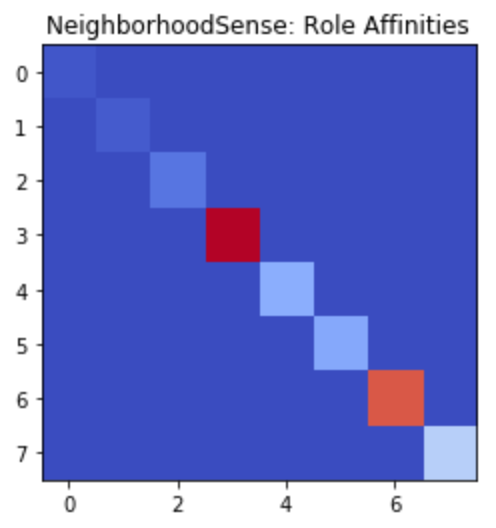
\includegraphics[width=0.75\linewidth]{neighborhoodsense.png}
    \caption{Role affinities computed by decomposing averaged neighborhood roles with user roles.}
    \label{fig:neighborhood_sense}
\end{figure}

\begin{figure}
    \centering
    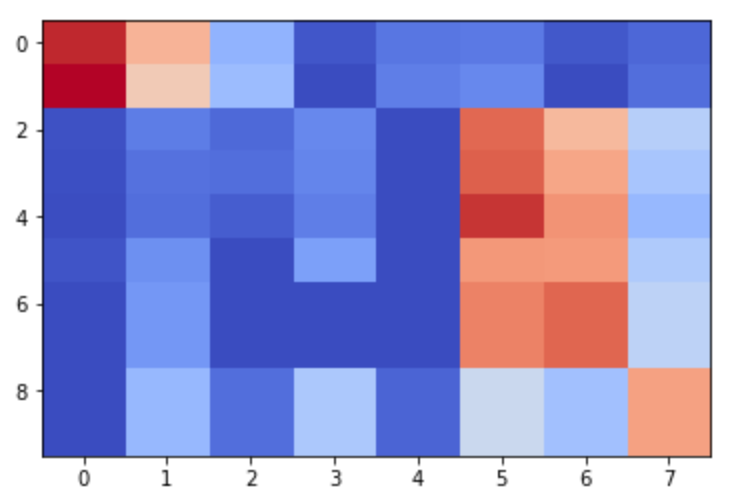
\includegraphics[width=0.75\linewidth]{top10-community-roles.png}
    \caption{Distribution of roles within the top 10 communities.}
    \label{fig:top_roles}
\end{figure}

\section{Community Features}

% maybe have table for runtime on x nodes?
In order to justify community features, we must first define a generic, viable clustering method for each snapshot. Because users may contribute to a diverse set of articles, and articles themselves may not necessarily fall within a single community, we think that a probabilistic representation of community membership, such as AGM, makes sense. Unfortunately, runtimes for, AGMfit\cite{leskovec2016snap} were prohibitive, even for relatively small subsets of our projection graphs. We also tried Spectral Clustering, but ran into similar issues.

\begin{table}[ht]
    \centering
    \begin{tabular}{c|c|c|c|c}
    \toprule
        Algorithm & Data & Nodes & Edges & Runtime \\
         \midrule
        % a single clique, I dont have any logs from the ones that were larger than this one. 
        AGMfit & User & 437 & 436 & 9 minutes \\
        Spectral (1 cut) & SSBM & 20k & 150k & 1 hour \\
        Louvain & User & 2.43m & 35m & 42 seconds \\
        Louvain & Article & 13.6m & 89.7m & 539 seconds \\
         \bottomrule
    \end{tabular}
    \caption{Runtime for Clustering Algorithms}
    \label{tab:clustering_runtime}
\end{table}

In contrast, the Louvain algorithm scales remarkably well (Table~\ref{tab:clustering_runtime}), even for sampled projections with >100m edges. However, because bots and admins are highly active and connected, they form a dense ball in the initial stages of clustering. Almost all users, even those with low activity, will end up assigned to the ball unless they have a clear membership in some relatively dense community. For the default and most modifications of the Louvain algorithm, we mostly end up with a few giant communities. However, by trying all the options for modularity in the C++ implementation (using a reference\cite{campigotto2014generalized} for model explanation, since the source is sparsely documented), we discovered that the indeterminance model worked quite well, and discovered a large number of nontrivial communities.

For comparison, the original modularity definition from Blondel is:
\begin{equation}
    Q = \frac{1}{2m} \sum_{i,j} (A_{ij} - \frac{k_i k_j}{2m}) \delta (c_i,c_j)
\end{equation}
And the deviation to indeterminance\cite{campigotto2014generalized} is:
\begin{equation}
    Q_{DI} = \frac{1}{2m} \sum_{i,j} (A_{ij} - \frac{k_i+k_j}{n} + \frac{2m}{n^2}) \delta (c_i,c_j)
\end{equation}

Given the above limitations, we run the Louvain algorithm on both the user and article projections for each snapshot. For users, communities correspond to sets of editors who maintain a common set of articles, and for articles, they represent pages maintained by a common set of users.

To build community features $u_c$ for a given community in the user projection, simply average over community members. $M(c)$ is the set of all users in community c.
\begin{equation}
    u_c = \frac{1}{|M(c)|} \sum_{i \in M(c)} B_{i:}
\end{equation}
We then assign user features by community memberships $C_i^{(u)} = u_c$, when user i belongs to community c. This creates duplicate rows for all members of the same community. We also considered community interaction features, but in practice the vast majority of out-community edges link to the admin/robot cluster.

For a given article community, we compute features $v_c$ by averaging over neighboring users in the bipartite graph. This captures the average user interacting with the community. $M(c)$ is the set of all articles in community c. 
\begin{equation}
    v_c = \frac{1}{\sum_{a \in M(c)}|N(a)|} 
    \sum_{a \in M(c)}\sum_{i \in N(a)} B_{(i:)}
\end{equation}
We then assign to articles by community membership: $a_j = v_c$ when article j belongs to community c. Then, we average over neighboring articles for each user i, again using the bipartite graph:
\begin{equation}
    C_{(i:)}^{a} = \frac{1}{|N(i)|} \sum_{j \in N(i)} a_j
\end{equation}

Finally, we concatenate these together to form the final community features:
\begin{equation}
    C = \begin{bmatrix}
        C^{(u)} & C^{(a)}
    \end{bmatrix}
\end{equation}
Observe that this formulation is generic -- we reuse the baseline features.

\section{Results}

The baseline features improved significantly on the null model, as expected. However, we did not find formulations where our simple role and community features add significant predictive power. We averaged model scores over 5 runs, since small deviations would impact these results.

\begin{table}[ht]
    \caption{Feature Performance}
    \label{tab:logloss}
    \centering
    \begin{tabular}{l|l|l|l}
        \toprule
         Model & Classification & Regression & Full \\
         \midrule
         Null Model & .453 & 0 & 0 \\
         $y^{(p-1)}$ only & .408 & .301 & .213 \\
         Baseline & .345 & .358 & .382 \\
         Roles & .412 & .252 & .190 \\
         Communities & .419 & .083 & .069 \\
         B + C & .340 & .361 & .389 \\
         B + R & .345 & .364 & .386 \\
         R + C & .390 & .269 & .227 \\
         B + R + C & .339 & .368 & .392 \\
         \bottomrule
    \end{tabular}
\end{table}

%rework/rework graph, placeholder (for both reg/class)
%probably want to frame wrap these (and maybe others)
%should also have more details. frame this as our results are: here's an overall table, here's some interesting things about regression, here's some interesting things about classification.
For the regression problem, the previous y-value was extremely useful as a variable (see Figure~\ref{fig:yprev}).
\begin{figure}[ht]
    \centering
    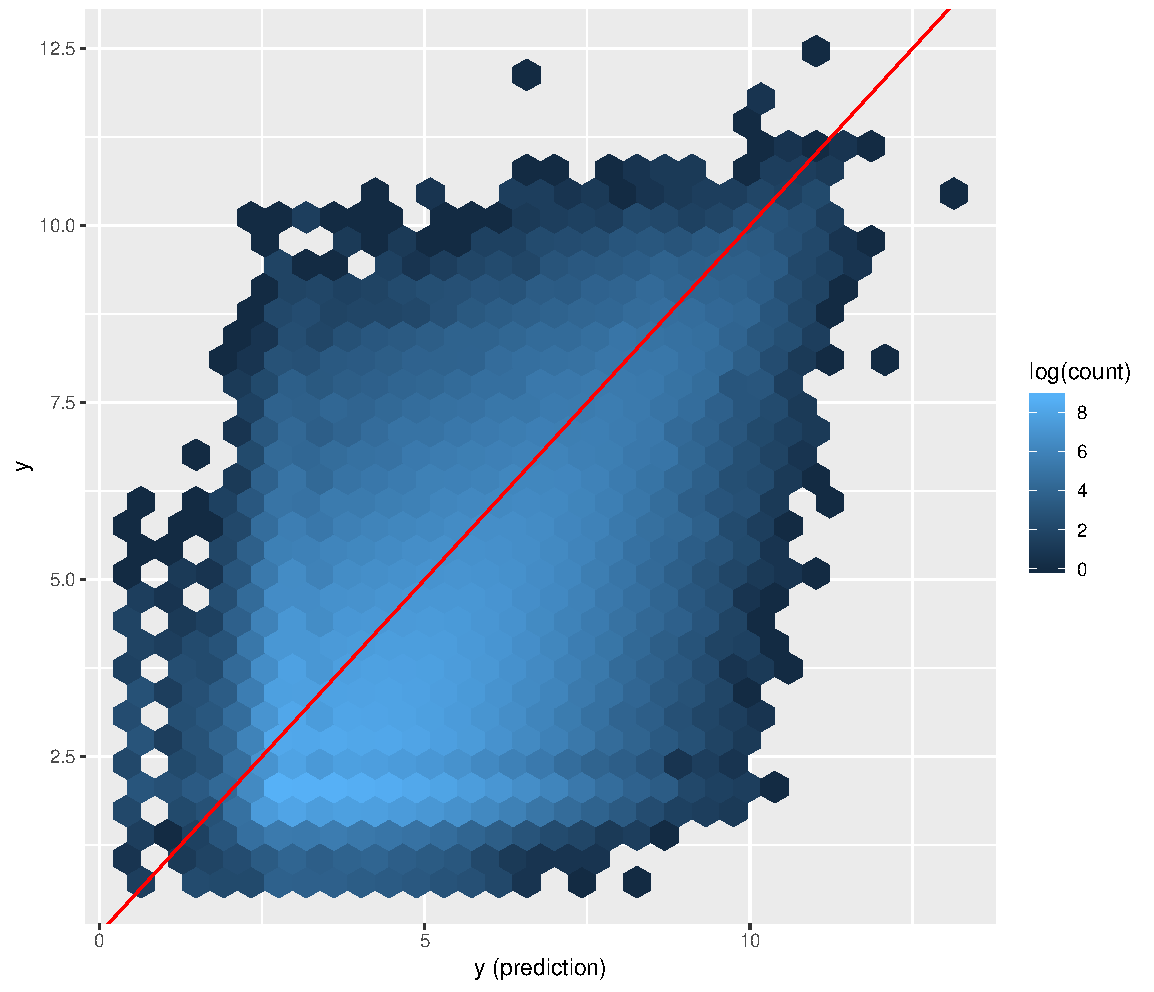
\includegraphics[width=1\linewidth]{prev_vs_target.pdf}
    \caption{Regression Performance, previous y value}
    \label{fig:yprev}
\end{figure}
However, we were still able to obtain significant improvement in the $R^2$ with our other features (see Figure~\ref{fig:yreg}). In general, many features added a small amount of improvement to the model.
\begin{figure}[ht]
    \centering
    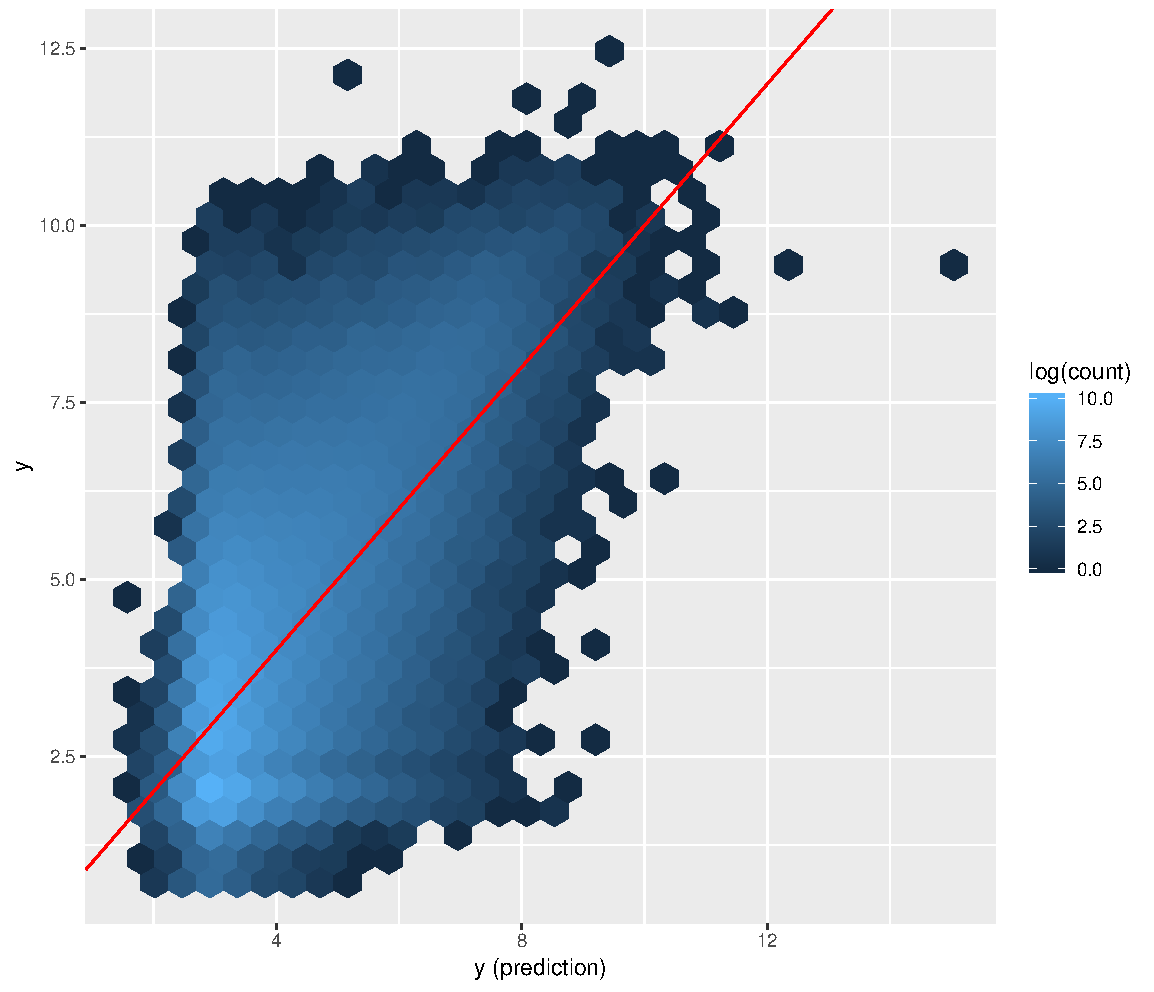
\includegraphics[width=1\linewidth]{reg_vs_target.pdf}
    \caption{Regression Performance, full model}
    \label{fig:yreg}
\end{figure}

For classification, the previous y-value was much less useful, relatively speaking. Much of the improvement from the baseline model stems from capturing better statistics about the population at a given time: for example, the retention rate is much higher in 2002 than in 2007. However, the community features only helped here to a limited extent due to the problems with our clustering implementation.
\begin{figure}[ht]
    \centering
    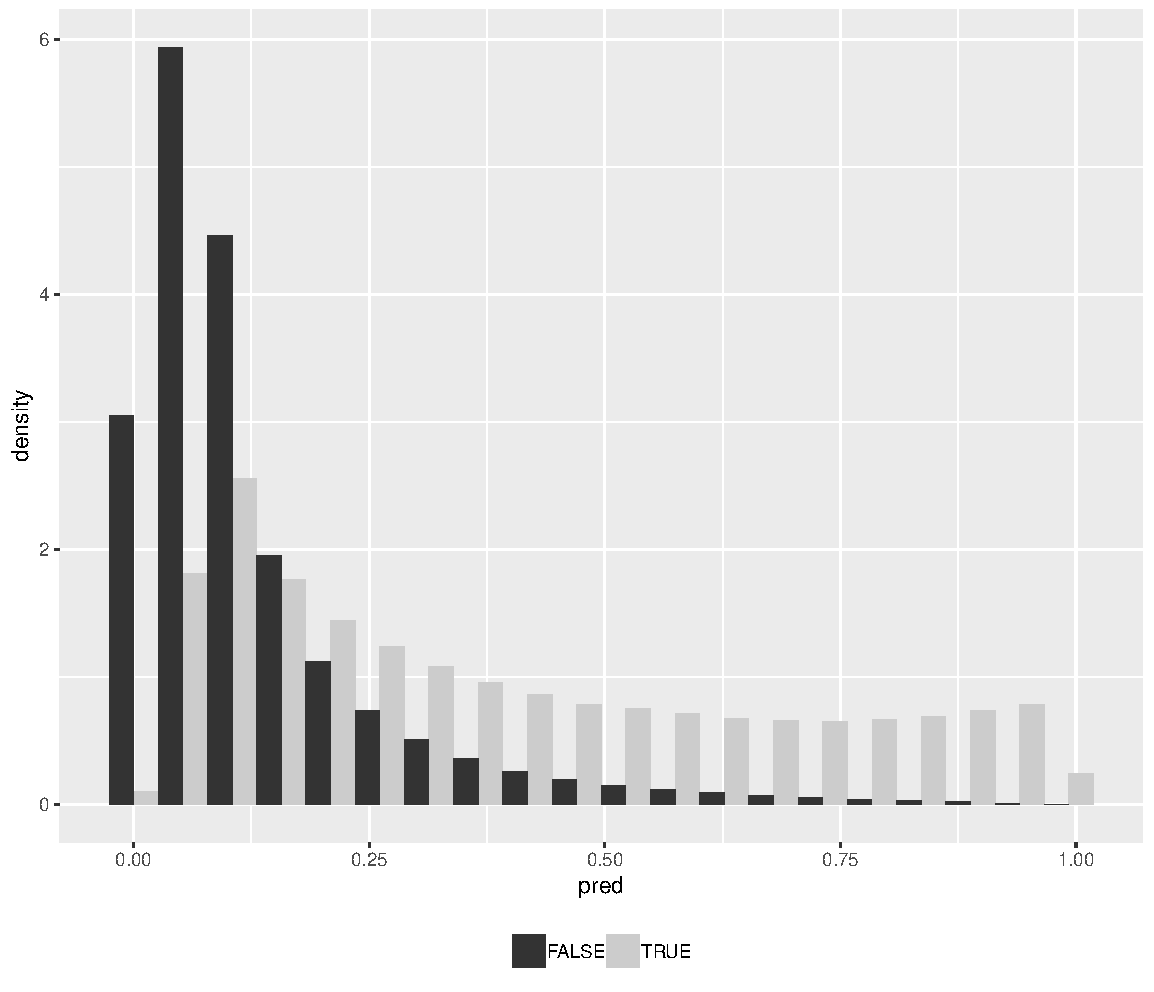
\includegraphics[width=1\linewidth]{class_full.pdf}
    \caption{Classification Performance}
    \label{fig:class_full}
\end{figure}

% define hedging
For the full model, we observe a hedging paradigm (Figure~\ref{fig:hedging}) because we cannot confidently classify that a given new user will participate in the next quarter, even if their contribution level is high. Thus, the model strikes a balance between underestimating users who do participate, and overestimating those who do not.
\begin{figure}[ht]
    \centering
    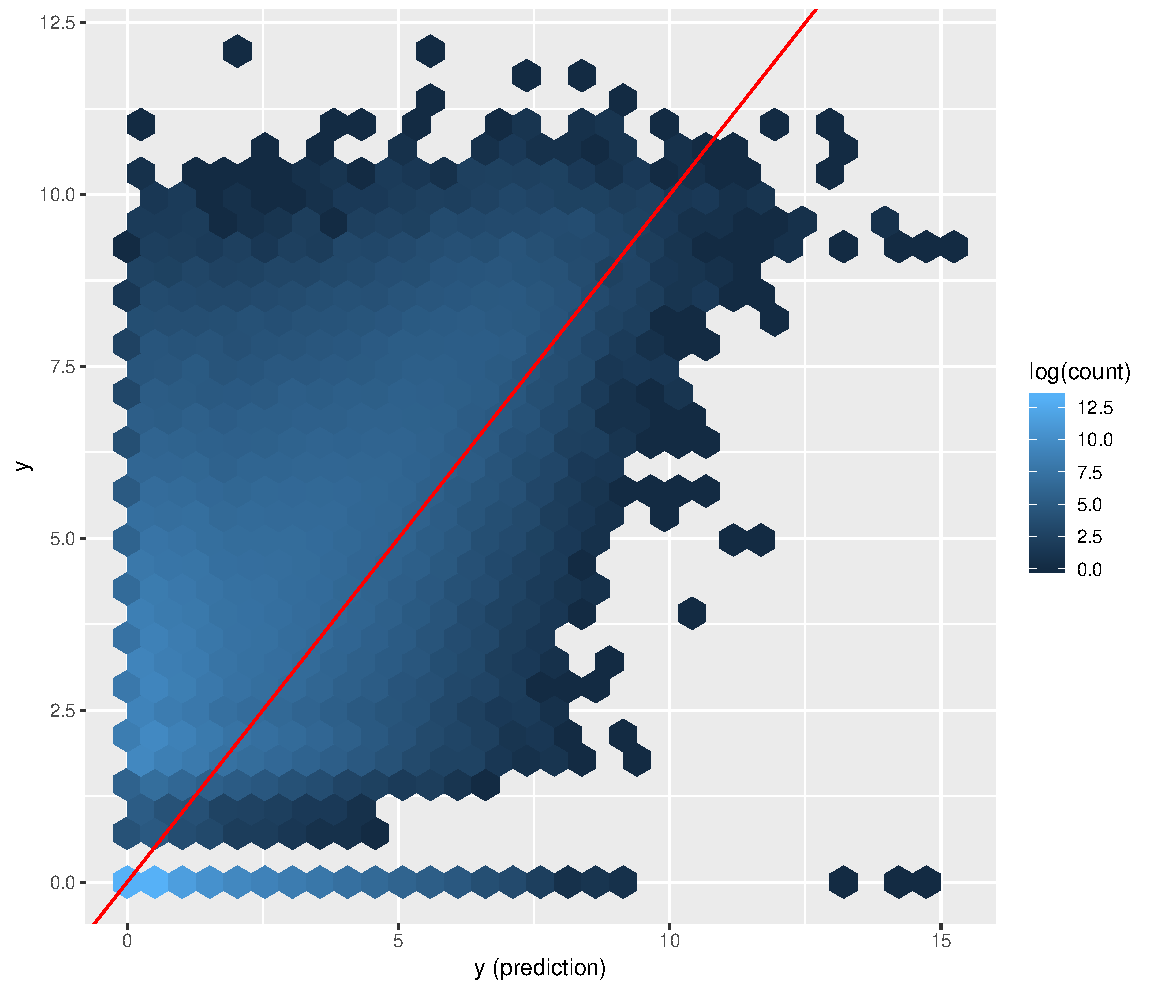
\includegraphics[width=1\linewidth]{reg_full.pdf}
    \caption{Full Model Performance}
    \label{fig:hedging}
\end{figure}

\section{Analysis}

To determine the most important features, we ran RFE for l2-regularized linear and logistic regression on the regression (Table~\ref{tab:top_reg}) and classification (Table~\ref{tab:top_class}) subproblems. This helps us roughly estimate importance on the original neural net. Note that the log loss and $R^2$ scores for these simple models are fairly close to the best neural net model, so this is not unreasonable.
\begin{table}[ht]
    \centering
    \begin{tabular}{c|c|c|c}
        \toprule
        Rank & Feature & Type & logloss \\
         \midrule
        1 & Time since Last Activity & $B_U$ & .4088 \\
        2 & $y^{(p-1)}$ & $B_U$ & .3800 \\
        3 & Activity Interval Length & $B_U$ & .3706  \\
        4 & Article Community Size & $C$ & .3682  \\
        5 & Period Number & $B_U$ & .3613  \\
        6 & User Community Average & $C$ & .3610  \\
        7 & Article Community Average & $C$ & .3607 \\
        13 & SVD-1 & $R$ & .0001 \\
        47 & All Features & $B+R+C$ & .3567 \\
         \bottomrule
    \end{tabular}
    \caption{Top Classification Features}
    \label{tab:top_class}
\end{table}
\begin{table}[ht]
    \centering
    \begin{tabular}{c|c|c|c}
        \toprule
        Rank & Feature & Type & $R^2$  \\
         \midrule
        1 & $y^{(p-1)}$ & $B_U$ & .1619  \\
        2 & Percent Distinct Articles & $B_U$ & .1961 \\
        3 & Total Edits (Article) & $B_A$ & .1972 \\
        4 & Total Big Edits (Article) & $B_A$ & .1974 \\
        5 & Total Edits & $B_U$ & .2382  \\
        18 & Article Community Size & $C$ & .2881 \\
        19 & SVD-1 & $R$ & .2881  \\
        20 & User Community Size & $C$ & .2883  \\
        47 & All Features & $BRC$ & .2906 \\
         \bottomrule
    \end{tabular}
    \caption{Top Regression Features}
    \label{tab:top_reg}
\end{table}

For classification, we were able to construct a good model by simply knowing how long it has been since the user last logged in. 

The ordering, outside of the top few features, is fragile to small changes to any part of the model, and addition of new features. However, the top features are effective: just three, $y^{(p-1)}$, time since last activity and activity interval length produced a $R^2$ score of .355 on the full model. The top five from each subproblem (9 total) scored .377. The best model score was .392, so we can clearly construct a near optimal model from a small feature set.

We also observed that community features improved classification. The article clustering mostly binned articles into a giant community for each snapshot, so the average community size correlates strongly to the number of unique articles that quarter. This indirectly indicates the time period, which helps since Wikipedia retention rates decreased over time. Clustering on the user projection created a significant set of small, dense communities. These contained low rates of new users, but assignment outside of the ball strongly indicates future activity beyond. As a test, replacing the feature with a "1" for mid-sized communities and "0" otherwise lead to a similar improvement. This contributed to about half of the difference between B to B+C, and is the most significant result that demands a graph interpretation.

Role features were generally more effective than community features by themselves, but did not rank well in either RFE. The more sophisticated full model improves only marginally in the regression task. In order to improve the model significantly, we would expect to observe affinities between roles. For example, interactions between bots and new users could imply negative experiences. While we are able to distinguish between types of users in differently sized communities (Figure~\ref{fig:top_roles}), the types of structural roles we discover in this network are limited -- the role features can be compressed into two dimensions that explain $97\%$ of the variance across snapshots. Our model shows that these dimensions closely map to contribution level (which we already measure).

\section{Null Results}
Our initial framing used a classification problem, with logistic regression for inseparability and thresholding to separate contribution levels into "0" or "1". However, this mapping was flagged as unnatural since our variable is continuous. We also switched to a less interpretable model (neural nets) to allow for more complex models, since simple linear or logistic regression did not capture behavior well, and thus created an artificially easy baseline. 

We also faced substantial difficulties while using common neighbor thresholds, due to the high degree of connectivity in natural projection graphs. For example, in the user-user projection with a threshold of $>=2$, the K-Core decomposition of a quarterly snapshot (Figure~\ref{fig:kcore_2007_1}) finds a dense K=625 core. The snapshot also has an effective network diameter is 2.8. This limits the usefulness of role discovery, since users generally filter in two buckets that roughly map to existing baseline features: high connectivity for lots of contributions and low connectivity otherwise. Similarly, in the community case, large cliques obscure the borders between neighborhoods where high activity users connect to each other in one giant semi-clique (C>0.5). Thresholding only accentuates the problem, since limited activity users are often completely disconnected from the network. This suggests that we cannot resolve this issue by modifying the threshold, since we will merely reduce the size of the ball.

\begin{figure}[ht]
    \centering
    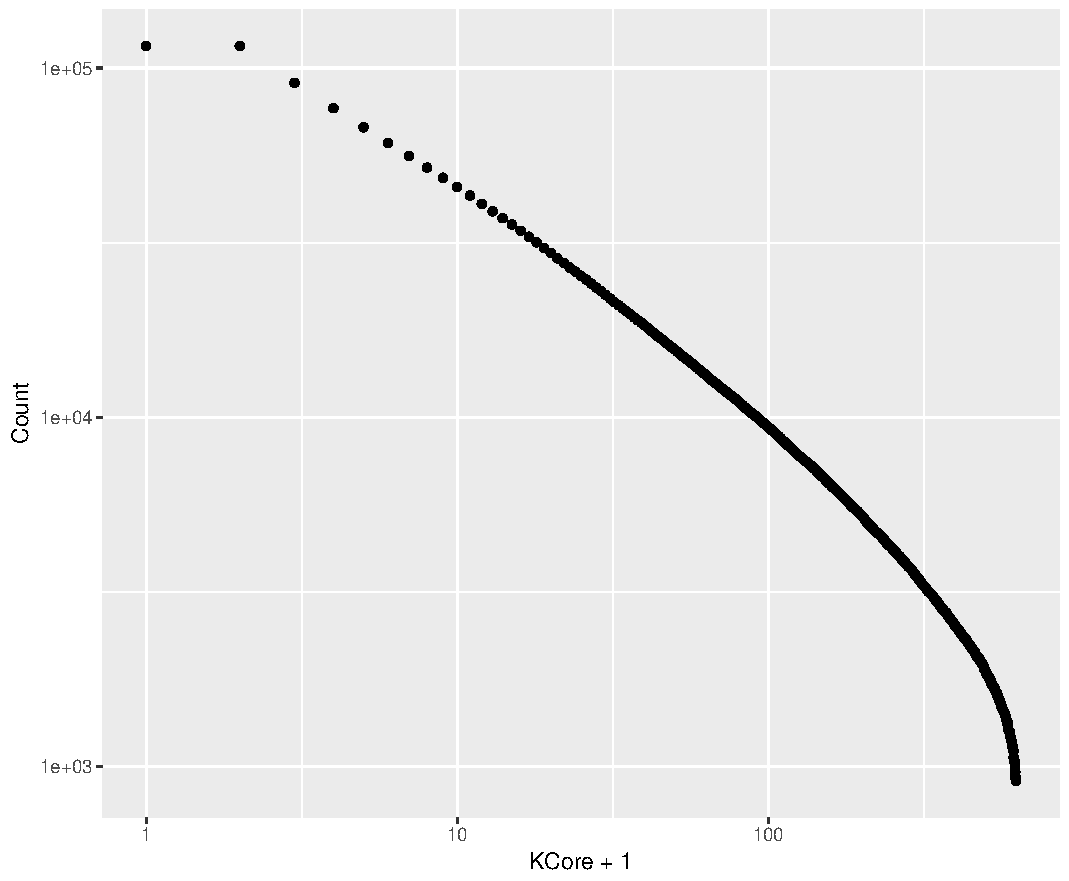
\includegraphics[width=1\linewidth]{kcore_dist_2007_1.pdf}
    \caption{KCore Distribution, 2007-Q1}
    \label{fig:kcore_2007_1}
\end{figure}

We also found that interactions within small time windows poorly describe Wikipedia activity, especially in comparison to other sites like StackOverflow. Cleanup in particular tends to happen either slowly over time, or during thematic exercises for a topic. As evidence of this, we modified the user-user projection so that users share an edge if they edit the same article within a small block of time. This generates a k-clique when k users edit the same article within the block. We intended to use this method to thin the high density regions of the base user-user projection, and capture actual interactions between users. However, even for expansive definitions of "small", such as one day, the vast majority of cliques were of size 1 (nobody else edited the article on the same day), which generates no edges and disconnects most new users.

For both roles and communities, we were interested in looking at projections on the entire graph, since this promised a better representation of long term user types and community structures. However, in both cases we ran into data leakage issues that improperly improved the model. For roles, running RolX over the whole graph somewhat approximated the users total contribution. Given their initial and total contributions, we can make strong inferences about activity in their second quarter. For communities, clustering on the whole graph generated many dense groups with about 50-200 users. Membership in one of these groups was a strong indicator of future contribution, since being assigned to one requires substantial activity. In both cases, we observed $R^2 > .5$ and extremely poor performance on the combined model.

\section{Future Work}

% analysis of existing users as opposed to acquisition; existing users have more information
% analysis of links formed by user-talk pages and communities across article hyperlinks as a more direct network, with the same types of techniques (structure + communities + sampling)

We think our general recipe (Algorithm~\ref{alg:ml}) has promise for generating nontrivial baseline prediction models on large k-partite graphs, and evaluating the information added by a graph-based approach. It certainly worked in our case, by rejecting most of our role and community feature sets. However, community detection requires a lot of custom modifications. Generalizing that process for projections would certainly prove useful across a wide variety of applications.

Also, our density reduction approach generalizes well for graphs that naturally generate large cliques, such as unimodal projections and citation networks. We particularly note the theoretical results for bounding the chance of disconnecting users. We also roughly preserve the proportions of the original degree distribution for projections, which may be desirable.

\section{Source Code}
All source code for this report can be found at \url{https://github.com/cs224w-f18-wikipedia-retention/wikipedia-retention}

\printbibliography[title={References}]

\end{document}